\documentclass[]{report}
\usepackage{graphicx}

% Title Page
\title{Report First project Big Data}
\author{Luca De silvestris (486652), Luca Polidori (488434)\\ Group name: DesiDori}


\begin{document}
\maketitle

\chapter*{assignment}
Si consideri il dataset Daily Historical Stock Prices, scaricabile dal sito del corso, che contiene l’andamento giornaliero
di un’ampia selezione di azioni sulla borsa di New York (NYSE) e sul NASDAQ dal 1970 al 2018. Il dataset è formato da
due file CSV. Ogni riga del primo ha i seguenti campi:
\begin{itemize}
	\item ticker: simbolo dell’azione
	\item open: prezzo di apertura
	\item close: prezzo di chiusura
	\item adjclose: prezzo di chiusura “modificato” (potete trascurarlo)
	\item lowThe: prezzo minimo
	\item highThe: prezzo massimo
	\item volume: numero di transazioni
	\item date: data nel formato aaaa-mm-gg
\end{itemize}

Il secondo ha invece questi campi:
\begin{itemize}
	\item ticker: simbolo dell’azione
	\item exchange: NYSE o NASDAQ
	\item name: nome dell’azienda
	\item sector: settore dell’azienda
	\item industry: industria di riferimento per l’azienda
\end{itemize}

Progettare e realizzare in: (a) MapReduce, (b) Hive e (c) Spark:\\
\textbf{1.} Un job che sia in grado di generare, in ordine, le dieci azioni la cui quotazione (prezzo di chiusura) è cresciuta
maggiormente dal 1998 al 2018, indicando, per ogni azione: (a) il simbolo, (b) l’incremento percentuale, (c) il
prezzo minimo raggiunto, (e) quello massimo e (f) il volume medio giornaliero in quell’intervallo temporale.\\
\textbf{2.} Un job che sia in grado di generare, per ciascun settore, il relativo “trend” nel periodo 2004-2018 ovvero un
elenco contenete, per ciascun anno nell’intervallo: (a) il volume complessivo del settore, (b) la percentuale di
variazione annuale (differenza percentuale arrotondata tra la quotazione di fine anno e quella di inizio anno)
e (c) la quotazione giornaliera media. N.B.: volume e quotazione di un settore si ottengono sommando i
relativi valori di tutte le azioni del settore.\\
\textbf{3. }Un job in grado di generare coppie di aziende di settori diversi le cui azioni che, negli ultimi 3 anni, hanno
avuto lo stesso trend in termini di variazione annuale indicando le aziende e il trend comune (es. Apple, Fiat,
2016:-1\%, 2017:+3\%, 2018:+5\%).

\chapter*{First Job}
\section*{Variables and choices}
We have chosen to use the following variables to find the respective project specifications for the first job:
\begin{itemize}
	\item \textbf{Incremento Percentuale}: is calculated by taking for each ticker the value of close variable with minimum date (\textit{prz\_ini\_chiusura}), value of close with maximum date (\textit{prz\_fin\_chiusura}) and applying the following formula:
	\begin{center}
			((\textit{prz\_fin\_chiusura} - \textit{prz\_iniz\_chiusura}) / \textit{prz\_iniz\_chiusura})*100.
	\end{center}
	\item \textbf{prezzo minimo}: calculated by taking the min (low) for each ticker.
	
	\item \textbf{prezzo massimo raggiunto}: calculated by taking the Max(high) for each ticker.
	
	\item \textbf{volume medio giornaliero}: represented by the variable \textit{volume\_avg\_giornaliero} is calculated by taking for each ticker:\textit{ sum(volume)} / \textit{numero\_giorni.}
\end{itemize}

\section*{PseudoCode Map-Reduce and output}
[\textbf{1}]\textbf{Map}\begin{itemize}
	\item \textbf{[1.1]} for each record of the csv "historical\_stock\_prices" it performs the filtering of the rows based on the date field such that 1998 <= anno <= 2018;
	\item \textbf{[1.2]} return ticker, close, low, high, volume, data.	
\end{itemize}
[\textbf{2}]\textbf{Reduce} \begin{itemize}
	\item \textbf{[2.1]}For each resource of the map output group the actions for ticker
	\item \textbf{[2.2]} Calculates for each ticker the value of: incremento\_percentuale, prez\_min\_raggiunto, prez\_max\_raggiunto, volume\_avg\_giornaliero.
	\item \textbf{[2.3]}sort by the percentage increment field and take the first 10 actions
	\item \textbf{[2.4]}return ticker, incrementPercentuale, prezzoMin, prezzoMax, volumeAvg
\end{itemize}
\newpage
\begin{center}
	\begin{figure}[!htb]
		\hspace{-1 cm}
		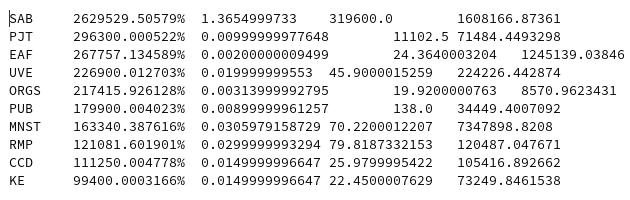
\includegraphics[width=1.2 \linewidth]{figure/output1map}
		\caption{output Job 1 Map Reduce}
	\end{figure}
\end{center}
\section*{PseudoCode Hive and output}
	\begin{itemize}
		\item[\textbf{1}] create table "prices" and upload data from the csv "\textit{historical\_stock\_prices.csv}
		\item[\textbf{2}] for filtering year from 1998 to 2018
		\item[\textbf{3}] final section of the fields: ticker, incremento percentuale, prezzo minimo, prezzo massimo 
		\item[\textbf{4}] grouping of the fields by ticker (by using \textit{Group by}) and by sorting according to "incrementoPercentuale" (by using \textit{Order by})
	\end{itemize}
\begin{center}
	\begin{figure}[!htb]
		\hspace{-1 cm}
		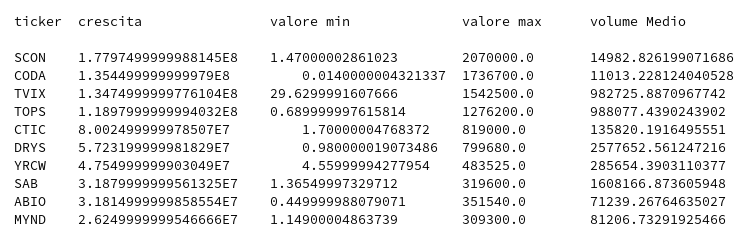
\includegraphics[width=1.2 \linewidth]{figure/output1hive}
		\caption{output Job 1 Hive}
	\end{figure}
\end{center}

\section*{PseudoCode Spark and output }
\begin{itemize}
	\item[\textbf{1}] csv loading and DataFrame "init" creation containing all the csv columns and adding the "year" column by processing the date field with filtering of the years> = 1998;
	\item[\textbf{2}] create dataFrames "prezzominimo","prezzomassimo" and "volumeGiornalieroMedio" starting from "init" dataframe and group by the ticker and adding respectively "prezzoMin", "prezzoMax" and "volumeMedio" columns;
	\item[\textbf{3}] join between dataframe and maximum, price by ticker and with the addition of the "incremento percentuale" column;
	\item[\textbf{4}] realization of the final dataframe with the addition of the column concerning the average daily volume and sorting by percentage increase.
\end{itemize}

\begin{center}
	\begin{figure}[!htb]
		\hspace{-2 cm}
		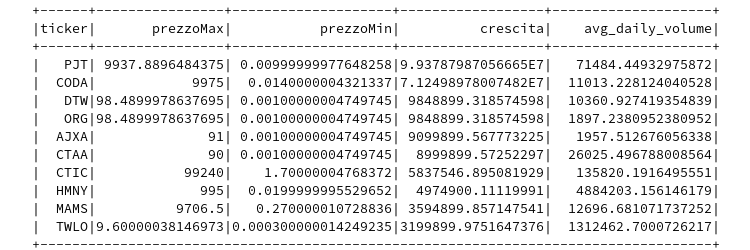
\includegraphics[width=1.4 \linewidth]{figure/output1spark}
		\caption{output Job 1 Spark}
	\end{figure}
\end{center}
\chapter*{Second Job}

\section*{Variables and choices}
We have chosen to use the following variables to find the respective project specifications for the second job:
\begin{itemize}
	\item \textbf{volume\_complessivo\_settore}: calculated for each sector and for each year by adding up all the volumes of the ticker;
	
	\item \textbf{quotazione\_giornaliera\_media}:calculated for each sector, for each year as the average of the sum of the relative values of that sector;

	\item \textbf{percentuale\_variazione\_annuale}: calculated for each sector, for each year by taking the sum of the close values with minimum date and same sector (\textit{prz\_ini\_chiusura}), the sum of the close values having maximum date and same sector (\textit{prz\_fin\_chiusura})and applying the following formula:
	\begin{center}
			((\textit{prz\_fin\_chiusura} - \textit{prz\_iniz\_chiusura}) / \textit{prz\_iniz\_chiusura})*100 
	\end{center}
	
\end{itemize}
\section*{PseudoCode Map-Reduce and output}
[\textbf{1}]\textbf{Map}\begin{itemize}
	\item \textbf{[1.1]}  for each record of the csv "historical\_stock\_prices" it performs the filtering of the rows based on the date field such that 2004 <= anno <= 2018;
	\item \textbf{[1.2]} return record, close, volume, data;
	\item \textbf{[1.3]} for each row of the csv historical\_stocks take the fields for ticker and sector;
	\item \textbf{[1.4]} maps the records obtained based on the ticker;
	\item \textbf{[1.5]} return sector, ticker, data, close, volume.
\end{itemize}
[\textbf{2}]\textbf{Reduce} \begin{itemize}
	\item \textbf{[2.1]}group tickers by sector and by year;
	\item \textbf{[2.2]}calculates the "volume\_complessivo","percentuale\_di\_variazione\_annuale", "quotazione\_giornaliera\_media";
	\item \textbf{[2.3]}return sector, anno, volume\_settore, percentuale\_di\_variazione,	quotazione\_giornaliera\_media.
\end{itemize}

\begin{center}
	\begin{figure}[!htb]
		\hspace{-1 cm}
		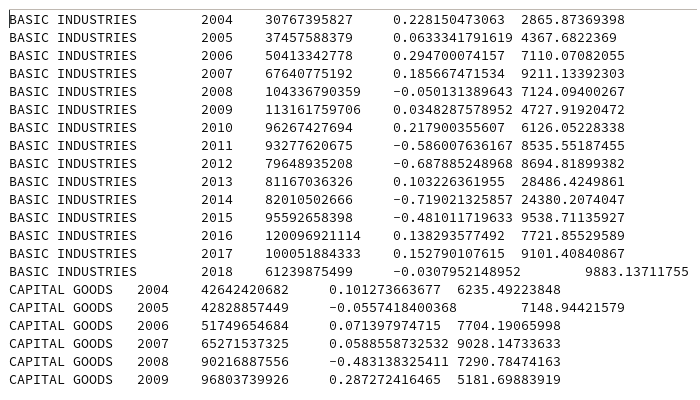
\includegraphics[width=1.2 \linewidth]{figure/output2map}
		\caption{output Job 2 Map Reduce}
	\end{figure}
\end{center}

\section*{PseudoCode Hive and output}
	\begin{itemize}
	\item[\textbf{1}] create table "prices" and "stock" and uploading data of the relative csv "\textit{historical\_stock\_prices.csv}" and "\textit{historical\_stocks.csv}";
	\item[\textbf{2}]  create table of joins between prices and stock tables with "ticker" as join condition with field selection: ticker, close, volume, data and sector and filtering year since 2004;
	\item[\textbf{3}] create table "sumOfVolume" for exclusive calculation of the "volume\_complessivo\_settore" variable by grouping the table by sector and year;
	\item[\textbf{4}] create table "DateMinMax" containing for each sector, ticker, year the "mindate" and the "maxdate";
	\item[\textbf{5}] create tables "minClose" e "maxClose" containing for each sector and year the sum("close") variable for each ticker with the condition "date"== "mindate" (for minClose table) and "date"=="maxdate" (for maxClose table);
	\item[\textbf{6}] create table "percentualeVariazione" having the fields sector, year and "variazione\_annuale" sorted by sector and by year;
	\item[\textbf{7}] create table "quotazione\_giornaliera\_media" which takes the average of the sum of the closing values for each sector and year
	\item[\textbf{8}] final query is the selection of the required fields FROM tabbles "quotazione\_giornaliera\_media", "percentualeVariazione" and "sumOfVolume" with the conditions for the sector and the year.
\end{itemize}
\begin{center}
	\begin{figure}[!htb]
		\hspace{-1 cm}
		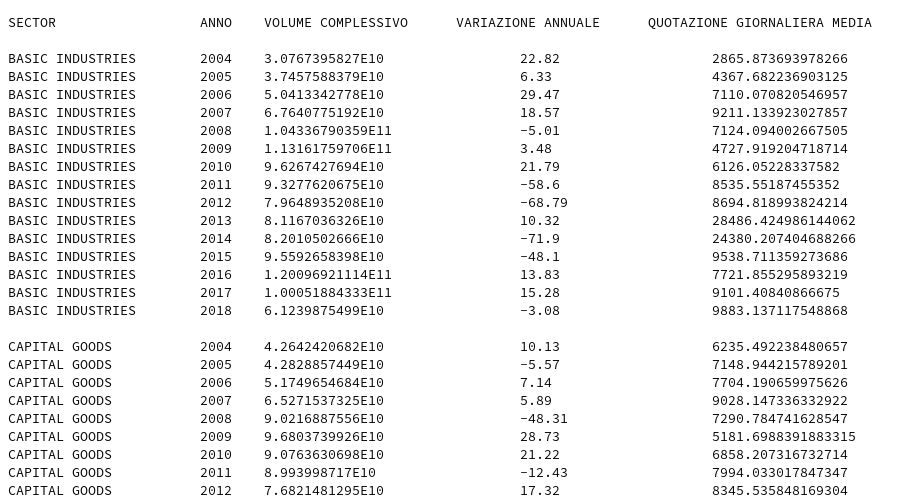
\includegraphics[width=1.3 \linewidth]{figure/output2hive}
		\caption{output Job 2 hive}
	\end{figure}
\end{center}

\section*{PseudoCode Spark and output}
\begin{itemize}
	\item[\textbf{1}] upload csv and create dataframe doc1 and doc2 containing all the columns of the respective csv;
	\item[\textbf{2}]  creation of join dataframes with addition of the "year" column and filtering YEAR> = 2004;
	\item[\textbf{3}] create dataframe "volumeComplessivo" for calculate "volume\_complessivo\_settore" grouping by sector and year;
	\item[\textbf{4}] create dataframe "DateMinMax" containing for each sector, ticker, year the minimum\_date and the maximum\_date;
	\item[\textbf{5}] create dataframe containing the sum of the closing prices grouping by sector, year and date;
	\item[\textbf{6}] create dataframe "a" e "b" containing for each sector and year the sum("close") of each ticker of a given sector with date == minimum\_date (for a) or date == maximum\_date (for b);
	\item[\textbf{7}] create dataframe for "percentualeVariazione" variable with the fields sector, year and "percentuale\_variazione\_annuale" sorted by sector and by year;
	\item[\textbf{8}] create final dataframe containing sector,year,"percentuale\_variazione\_annuale", "volume\_complessivo\_settore" and "quotazione\_media\_giornaliera" sorted by sector and by year by merging the relevant columns of the previous data frames created.
\end{itemize}
\begin{center}
	\begin{figure}[!htb]
		\hspace{1.3 cm}
		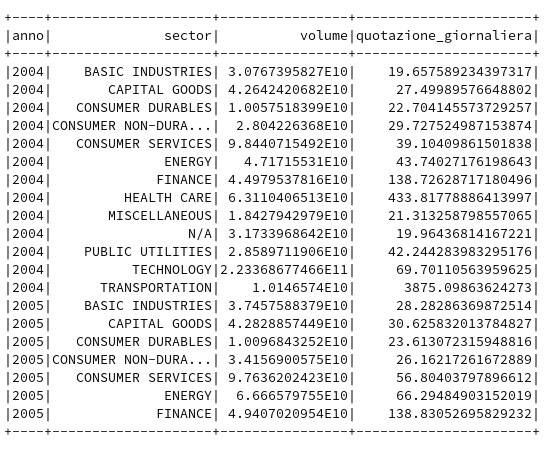
\includegraphics[width=0.8 \linewidth]{figure/output2spark}
		\caption{output Job 2 Spark}
	\end{figure}
\end{center}


\chapter*{Third Job}

\section*{Variables and choices}
We have chosen to use the following variables to find the respective project specifications for the third job:
\begin{itemize}
	\item \textbf{percentuale\_variazione\_annuale} calculated for each sector, for each year and for each name by taking the value of close with minimum date (\textit{prz\_ini\_chiusura}), value of close with maximum date (\textit{prz\_fin\_chiusura}) and applying the following formula:
	\begin{center}
		((\textit{prz\_fin\_chiusura} - \textit{prz\_iniz\_chiusura}) / \textit{prz\_iniz\_chiusura})*100 
	\end{center}
	
\end{itemize}


\section*{PseudoCode Map-Reduce and output}
[\textbf{1}]\textbf{Map}\begin{itemize}
	\item \textbf{[1.1]}  for each record of the csv "historical\_stock\_prices" it performs the filtering of the rows based on the date field such that 2016 <= anno <= 2018;
	\item \textbf{[1.2]} return ticker, close e date;
	\item \textbf{[1.3]} for each record of the csv historical\_stocks retrieve the fields related to the ticker, name and sector;
	\item \textbf{[1.4]} combines records based on the ticker;
	\item \textbf{[1.5]} return name, date, sector, close;
\end{itemize}
[\textbf{2}]\textbf{Reduce} \begin{itemize}
	\item \textbf{[2.1]}groups ticker by name, year
	\item \textbf{[2.2]}for each year and for each company name calculates the  "percentuale\_variazione \_annuale" rounded to the int part.
	\item \textbf{[2.3]}for each company, emit the trend that "percentuale\_variazione\_annuale", name,sector for the last tree years.
\end{itemize}
[\textbf{3}]\textbf{Map}\begin{itemize}
	\item \textbf{[3.1]} load reduce's output.
\end{itemize}
[\textbf{4}]\textbf{Reduce} \begin{itemize}
	\item \textbf{[4.1]}check company trends;
	\item \textbf{[4.2]}issue company pairs with the same trend, such that the company belongs to different sectors.
\end{itemize}

\begin{center}
	\begin{figure}[!htb]
		\vspace{1 cm}
		\hspace{-4.7 cm}
		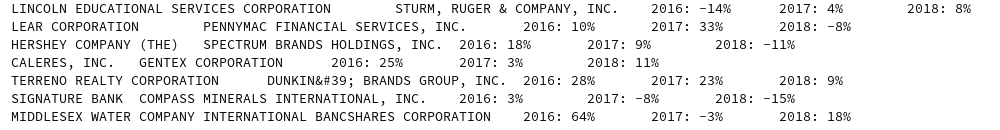
\includegraphics[width=1.8 \linewidth]{figure/output3map}
		\caption{output Job 3 Map Reduce}
	\end{figure}
\end{center}


\section*{PseudoCode Hive and output}
	\begin{itemize}
	\item[\textbf{1}] create table "prices" and "stock" and uploading data of the relative csv "\textit{historical\_stock\_prices.csv}" and "\textit{historical\_stocks.csv}";
	\item[\textbf{2}] create table of joins between prices and stock tables with "ticker" as join condition with field selection: ticker, close, volume, data and sector and filtering year since 2016;
	\item[\textbf{3}]  create dataframe "DateMinMax" containing for each sector,name, ticker, year the minimum\_date and the maximum\_date;
	\item[\textbf{4}] create tables "minClose" e "maxClose" containing for each sector,name and year the sum("close") variable for each ticker with the condition "date"== "mindate" (for minClose table) and "date"=="maxdate" (for maxClose table);
	\item[\textbf{5}] create table "percentuale" with the fields name, sector, year e "percetuale\_variazione\_annuale" sorting by name,sector and year;
	\item[\textbf{6}] create table "finalTable" and take name1,name2,year,"percentuale\_variazione\_annuale" FROM 2 tables "percentuale" renamed n1 and n2 with conditions: n1.name!=n2.name, n1.sector!=n2.sector, n1.anno==n2.anno e n1." percentuale\_variazione\_annuale" = n2."percentuale\_variazione\_annuale" 
	\item[\textbf{7}] final query is the selection of the required fields FROM tree tables "finalTable"  with conditions for name and years and sort by "name1" and "name2".
\end{itemize}

\begin{center}
	\begin{figure}[!htb]
		\hspace{-3 cm}
		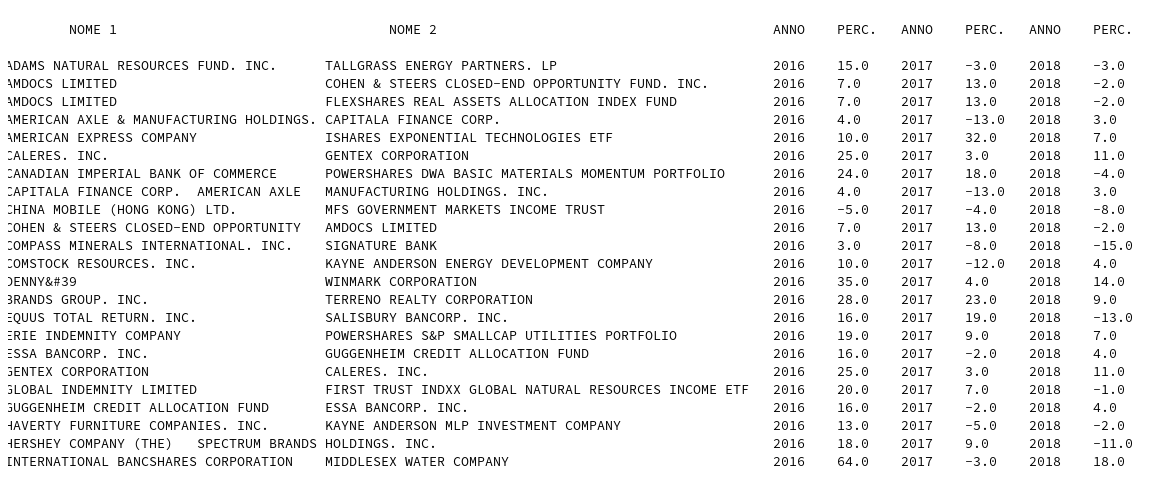
\includegraphics[width=1.5 \linewidth]{figure/output3hive}
		\caption{output Job 3 Hive}
	\end{figure}
\end{center}
\newpage
\section*{PseudoCode Spark and output}
\begin{itemize}
	\item[\textbf{1}] upload csv and create dataframe doc1 and doc2 containing all the columns of the respective csv;
	\item[\textbf{2}] creation of join dataframes with addition of the "year" column and filtering YEAR> = 2016;
	\item[\textbf{3}] create dataframe "DateMinMax" containing for each sector, ticker, year the minimum\_date and the maximum\_date;
	\item[\textbf{4}] create dataframe "a" e "b" containing for each sector and year the sum("close") of each ticker of a given sector with date == minimum\_date (for a) or date == maximum\_date (for b);
	\item[\textbf{5}] create dataframe for "percentualeVariazione" variable with the fields sector,name, year and "percentuale\_variazione\_annuale" sorted by sector and by year;
	\item[\textbf{6}] create final dataframe like cross-join of 2 dataframe "percentualeVariazione" with conditions: different name, different sector, same year and same "percentuale\_variazione\_annuale".
\end{itemize}

\begin{center}
	\begin{figure}[!htb]
		\vspace{1 cm}
		\hspace{-1 cm}
		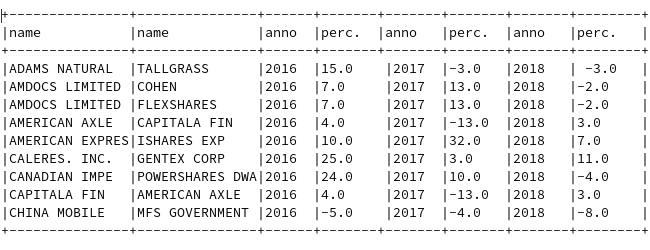
\includegraphics[width=1.2 \linewidth]{figure/output3spark}
		\caption{output Job 3 Spark}
	\end{figure}
\end{center}


\chapter*{Execution times and statistics}
To testing the timing of various jobs and various technologies have been used plus csv. In particular, the csv "historical\_stock\_prices.csv" was also halved and reduced to a third, thus creating copies with input for testing variable variables and allocating them for delivery.

\subsection*{Map reduce vs. Hive vs. Spark}
\begin{center}
\begin{figure}[!htb]
		\hspace{-1cm}
		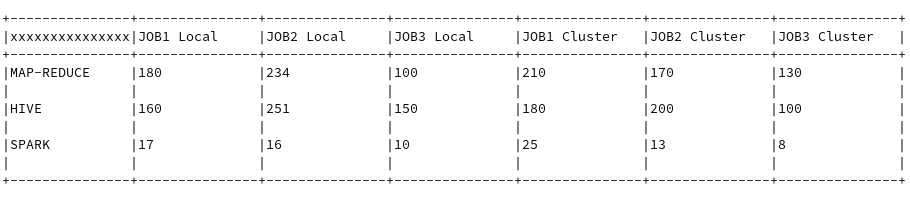
\includegraphics[width=1.2 \linewidth]{figure/valori}
		\caption{execution time in seconds}
\end{figure}
\end{center}
The various times reported for the Hive and Spark technologies are also formed by the loading time of the CSV and in the case of the second and third exercise also by the time of Join of the two CSVs, which in particular worsens the execution time of Hive.
The big difference in execution times between Spark and the two other technologies can already be analyzed. This difference resolved even more evident going to make the "bar Charts" to compare the time as shown below.
\newpage
\begin{center}

\begin{figure}[!htb]
	\hspace{-2.3 cm}
	\vspace{1.5 cm}
	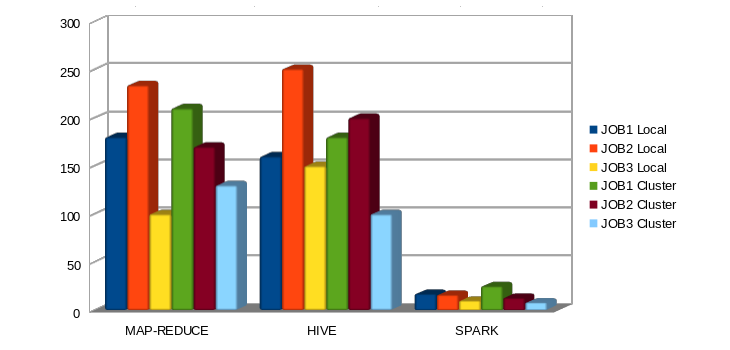
\includegraphics[width=1.5 \linewidth]{figure/grafico1}
\end{figure}
\end{center}

As mentioned, the CSVs have been divided and partitioned to take note of the execution times on several inputs.
The following are the times and barcharts for each csv and for each job of all technologies.\\
\newpage
\subparagraph*{Spark execution time}
\begin{center}
	\begin{figure}[!htb]
		\begin{minipage}[c]{.40\textwidth}
			\vspace{2 cm}
			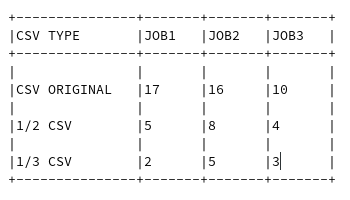
\includegraphics[width=1.2 \linewidth]{figure/sparktime}
			\caption{Time in second for spark}
		\end{minipage}
		\begin{minipage}{.40\textwidth}
			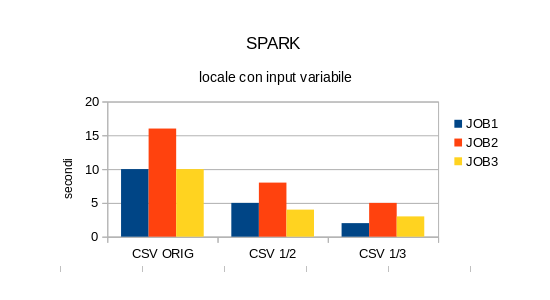
\includegraphics[width=2.3 \linewidth]{figure/sparkchart}
		\end{minipage}
	\end{figure}
\end{center}

\subparagraph*{Hive execution time}
\begin{center}
	\begin{figure}[!htb]
		\begin{minipage}[c]{.40\textwidth}
			\vspace{2 cm}
			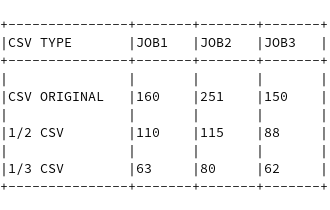
\includegraphics[width=1 \linewidth]{figure/hivetime}
			\caption{Time in second for Hive}
		\end{minipage}
		\begin{minipage}{.40\textwidth}
						\hspace{1 cm}
			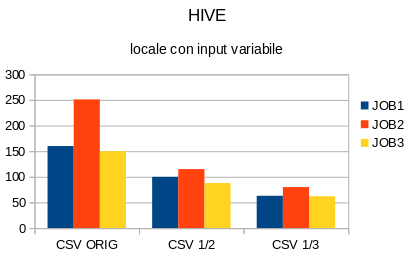
\includegraphics[width=2 \linewidth]{figure/hivechart}
		\end{minipage}
	\end{figure}
\end{center}	
\newpage
\subparagraph*{Map Reduce execution time}
\begin{center}
	\begin{figure}[!htb]
		\begin{minipage}[c]{.40\textwidth}
			\vspace{2 cm}
			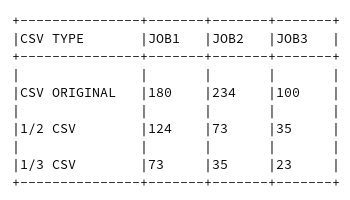
\includegraphics[width=1 \linewidth]{figure/maptime}
			\caption{Time in second for Map Reduce}
		\end{minipage}
		\begin{minipage}{.40\textwidth}
						\hspace{0.1 cm}
			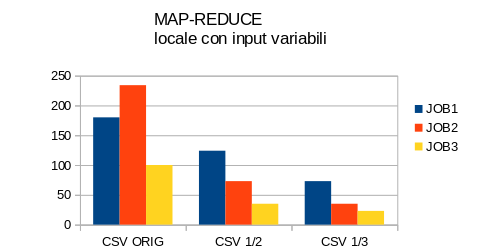
\includegraphics[width=2.4 \linewidth]{figure/mapchart}
		\end{minipage}
	\end{figure}
\end{center}	
	
	
\end{document}          
